\chapter{Electric Dipole Moment of Leptons}
\label{ch:leptonEDM}

Naturally, following the framework laid out previously, we want to perform calculations on the various leptons.
A brief review of past experimental results shows that the experimental development of electron EDM (eEDM) over the past few years has been remarkably rapid.
Just earlier last year, JILA~\cite{JILA23} has surpassed the previous bound from ACME~\cite{ACME18} and pushed the precision of eEDM down to \(|d_{e}| < 4.1 \times 10^{-30}\) \(e\,\mathrm{cm} \).
It is noteworthy to point out that these eEDM experiments are relatively small in scale, ``tabletop experiments'' even when compared to behemoths like the LHC, which makes the extreme precision achieved all the more impressive.
For the electron, an extensive study of eEDM in {\gthdm} can be found in the 2018 and 2020 papers of Fuyuto, Senaha, and Hou (Refs.~\cite{FSH20}).
Our investigation on eEDM is essentially an extension of the 2020 paper to a larger parameter space.

As mentioned before, one big motivation for {\gthdm} as a viable model is the fact that \(\order{1} \rho_{tt}\) can drive baryogenesis through \(\lambda_{t}\Im\rho_{tt} \).
However, this same \(\rho_{tt} \), along with \(\rho_{ff} \) for a given fermion \(f \), also generates EDM for said fermion.
We thus arive at a ``point of tension'' between theory and experiment:
we desire a large \(\rho_{tt} \) for baryogenesis, but need a small \(\rho_{tt} \) to survive precision bounds on various EDMs.
Electron EDM, in particular, is a great ``observable of contention'', since experiments measuring it are the most precise compared to other EDMs.
In an attempt to address this issue, Fuyuto, Senaha, and Hou proposed a ``cancellation ansatz'' between \(\rho_{ee} \) and \(\rho_{tt} \) 
\begin{equation}\label{eq:ansatz}
    \Re\rho_{ee} = -r\frac{\lambda_{e}}{\lambda_{t}}\Re\rho_{tt} \text{, } \quad \Im\rho_{ee} = +r\frac{\lambda_{e}}{\lambda_{t}}\Im\rho_{tt},
  \end{equation}
that allows for small values of eEDM while keeping a \textit{sizeable} \(\rho_{tt} \).
The \(r \) depends on the loop functions from the previous chapter.
This ansatz signifies two key points.
First, it gives a flavor hierarchy \(|\rho_{ee}|/|\rho_{tt}|\sim\lambda_{e}/\lambda_{t} \) that reflects SM.
Second, it represents a phase lock between \(\rho_{ee} \) and \(\rho_{tt} \).
This ansatz results in a ``dip'' in eEDM around the \(r \) value of \(\sim 0.7 \),
which is when the \(W \)-loop and the top-loop in the Barr-Zee diagram effectively cancel each other out.
This provides a mechanism for the eEDM in {\gthdm} to be small and evade the experimental bounds while not directly modifying \(\rho_{tt} \).
When revisiting their study, we found the assumptions on the value of \(\rho_{tt} \) to be quite ``conservative'', setting \(\Re\rho_{tt} = \Im\rho_{tt} = -0.1 \) (which equates to \(|\rho_{tt}| = 0.1\sqrt{2} \approx 0.14\)).
We believe that might be due to \textit{playing it safe} under the pressure of the rapid advancements on the experimental front. 
In our study~\cite{HKT23-2}, we \textit{push against the boundary}, and explore a larger range of \(\rho_{tt} \), up to \(\Re\rho_{tt} = \Im\rho_{tt} = -0.3 \) (\(|\rho_{tt}| = 0.3\sqrt{2} \approx 0.42\)). 
We want to see how big we can keep the parameter space for baryogenesis while still satisfying precision constraints.
As mentioned before, one of the key points of {\gthdm} is the \textit{flavor hierarchy}, illustrated by the \textit{rule of thumb}~\eqnref{eq:ruleofthumb}.
This ``cancellation ansatz'' happens to capture the idea of such a hierarchy pretty well from a numerical standpoint; 
so, for the sake of numerical illustration of the flavor hierarchy, we extend the ansatz to all fermion \(\rho_{ff} \)s, except for the top itself:
\begin{equation}\label{eq:ansatz-extended}
    \Re\rho_{ff} = -r\frac{\lambda_{f}}{\lambda_{t}}\Re\rho_{tt} \text{, } \quad \Im\rho_{ff} = +r\frac{\lambda_{f}}{\lambda_{t}}\Im\rho_{tt}.
\end{equation}
We must reiterate that this is merely a move of convenience, and the actual values of the \(\rho_{ff} \)s need not precisely match this ansatz.
Results are shown in \figref{fig:eEDM}.

\begin{figure}[t]
    \centering
    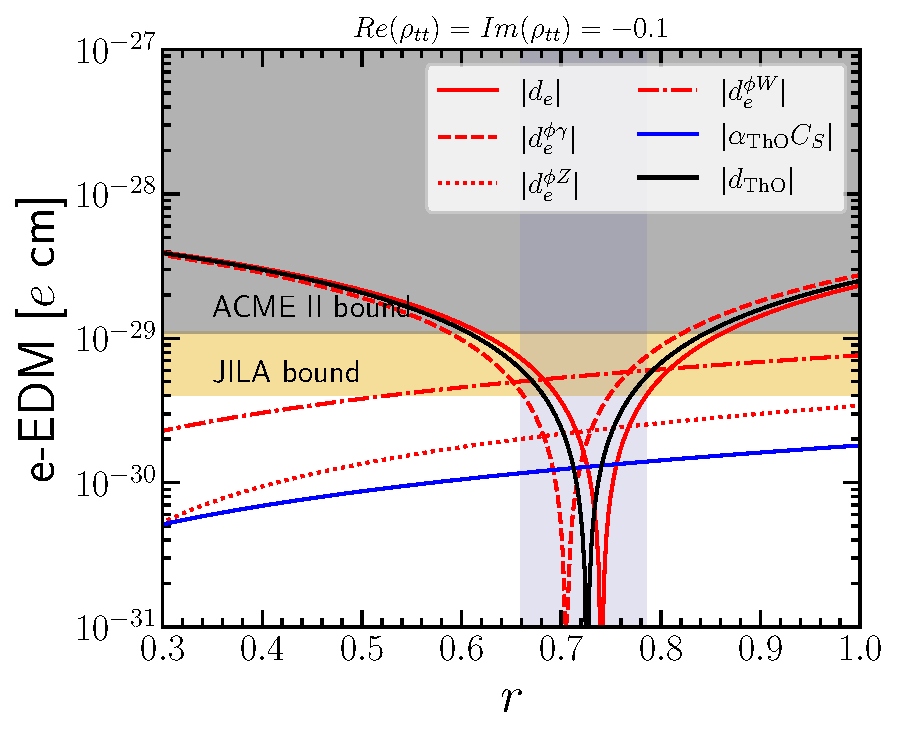
\includegraphics[width=5.3cm,height=3.7cm]{fig2_1.pdf}
    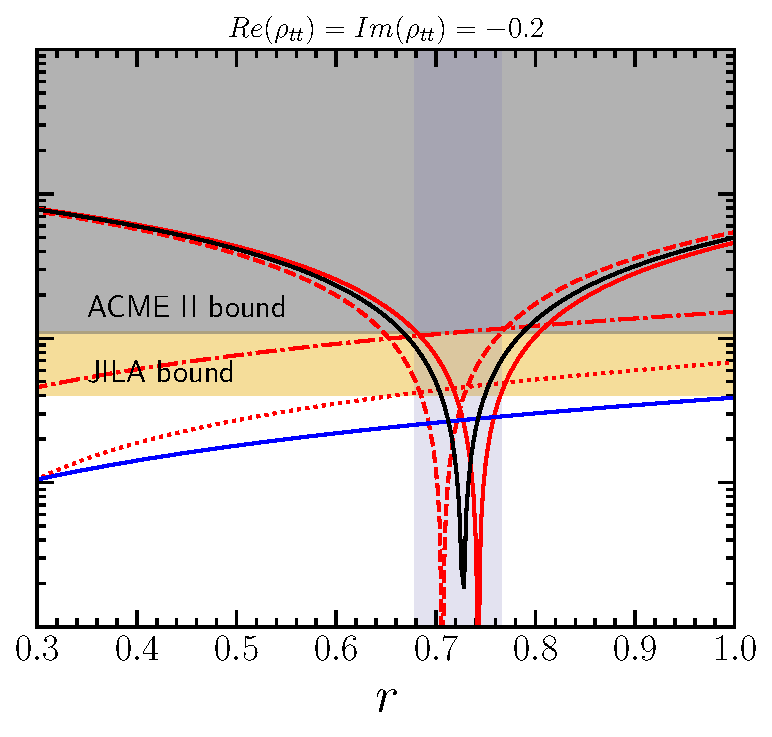
\includegraphics[width=4.63cm,height=3.7cm]{fig2_2.pdf}
    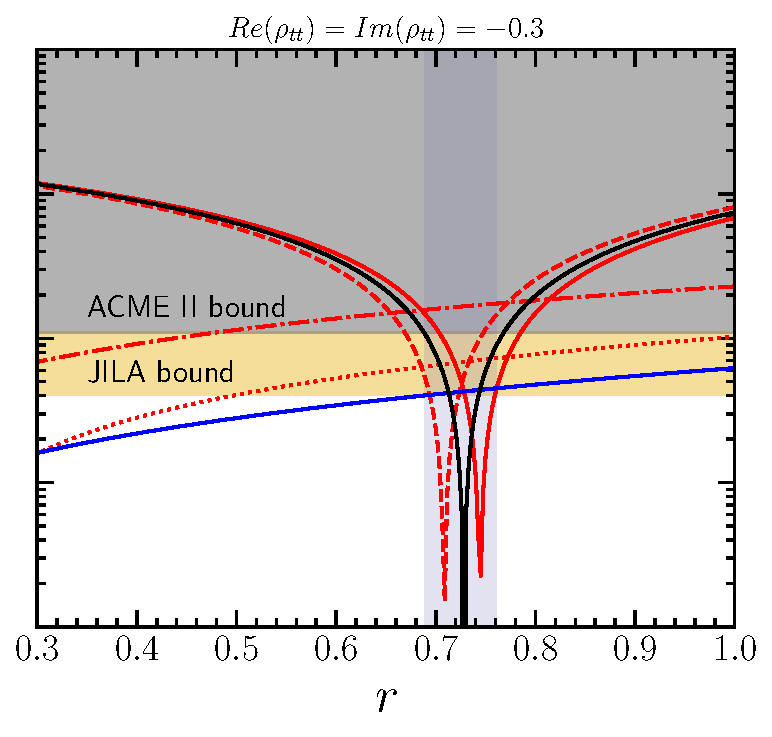
\includegraphics[width=4.63cm,height=3.7cm]{fig2_3.pdf}
    \caption{eEDM v.s. \(r \) for a larger range of \(\rho_{tt} \) with ansatz~Eq.~\eqref{eq:ansatz}. (\(c_{\gamma} = 0.1, m_{H, A, H^+} = 500\,\mathrm{GeV} \))}
    \label{fig:eEDM}
\end{figure}

For the sake of clarity, we have taken a slight liberty in illustrating the range of the purple ``allowed window'' band,
using the left- and right-most curves instead of the left and right side of a given curve.
Nevertheless, the trend we wish to describe is not affected by such.
From our results, it can be seen that as \(|\rho_{tt}| \) increases, the allowed window of the proportionality parameter \(r \) shrinks, yet there is still a decent range of acceptable probable values.
\(\Re\rho_{tt} = \Im\rho_{tt} = -0.1 \) was indeed a conservative representative value, and \(\Re\rho_{tt} = \Im\rho_{tt} = -0.3 \) may still be a viable option in the baryogenesis parameter space.

After the electron, we move on to its slightly heavier cousin, the muon. 

Lastly, we analyze the heaviest lepton, the tau. 
On the experiment front, the precision of tauEDM measurements are still pretty low.
As seen in \figref{fig:tauEDM}, when performing the same analysis as the muon, our predicted values are still several orders of magnitude below current experimental results.
Further precision or methodology improvements are required for a more fruitful analysis of tauEDM, so we just present our results here without much further comment.
